\section{Polarización en cd}

\subsection{BJT}
Un transistor debe ser apropiadamente polarizado con un voltaje de cd para que
opere como amplificador lineal. Se debe ajustar el punto de operación en cd de
modo que las variaciones de la señal en la terminal de entrada se amplifiquen y
reproduzcan con precisión en la terminal de salida. El punto de operación en cd
a menudo se conoce como \textbf{punto Q}.

Si un amplificador no se polariza con voltajes de cd correctos a la entrada y
salida, puede irse a saturación o a corte cuando se aplique una señal de
entrada.

La operación en cd de un circuito con un transistor se describe gráficamente con
una \textbf{recta de carga en cd}. Esta es una recta sobre las curvas
características desde el valor de saturación donde
$I_{\text{C}} = I_{\text{C(sat)}}$ sobre el eje $y$ hasta el valor de corte
donde $V_{\text{CE}} = V_{\text{CC}}$ sobre el eje $x$. El circuito externo
($V_{\text{CC}}$ y $R_{\text{C}}$) determina la recta de carga, no el transistor
mismo. El punto donde la recta de carga corta una curva característica
representa al punto Q con ese valor particular de $I_{\text{B}}$ \cite{Floyd}.

\subsubsection{Divisor de voltaje}
El método mas utilizado para la polarización del transistor es por medio de un
divisor de voltaje como se muestra en la \textbf{figura~\ref{figura11}}.

\begin{figure}[!ht]
\centering
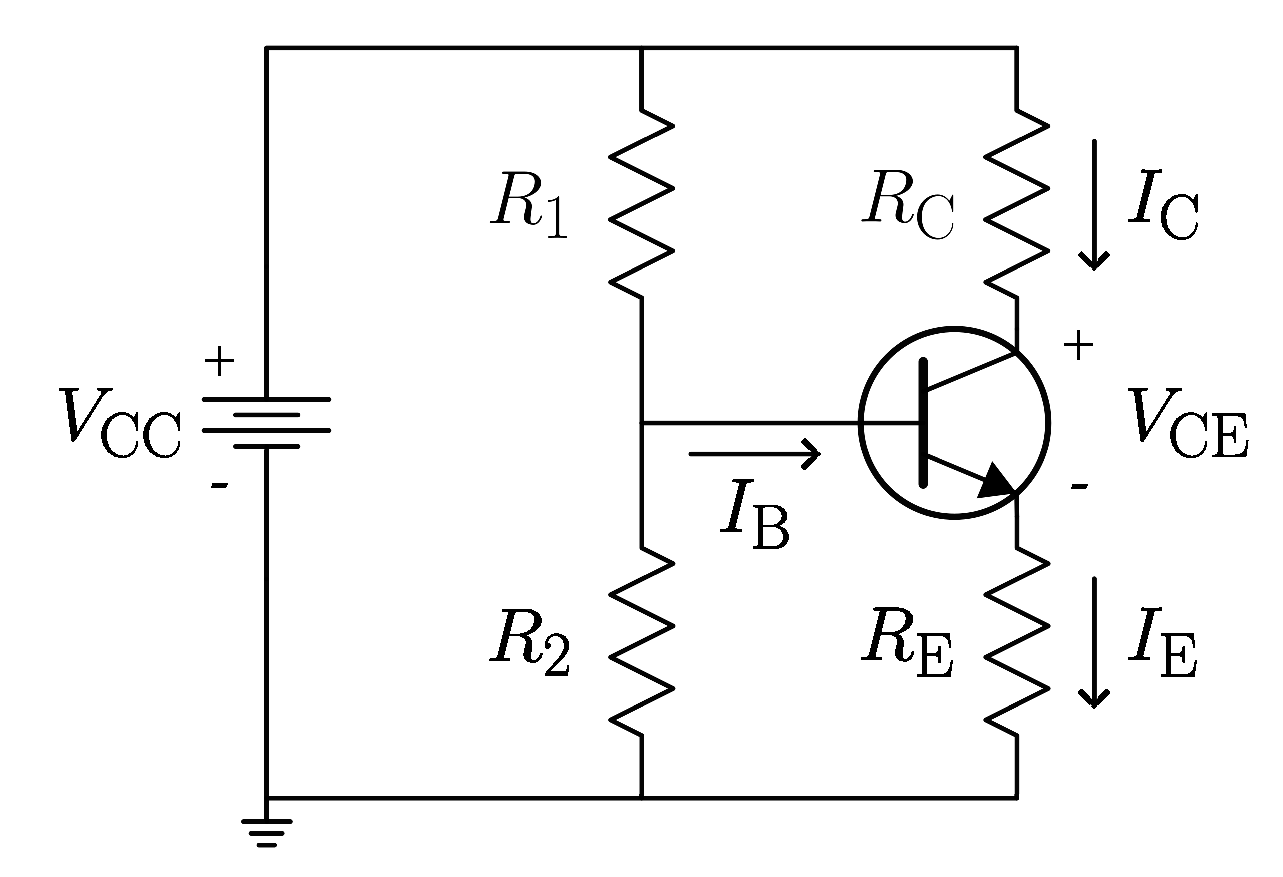
\includegraphics[scale=0.26]{diagramas/figura11.eps}
\caption{Circuito divisor de voltaje.}
\label{figura11}
\end{figure}

Para el calculo de los valores del circuito se utilizan las siguientes
ecuaciones \cite{Boylestad}:
\begin{equation*}
    \begin{split}
        R_{\text{TH}} &= \frac{R_1\,R_2}{R_1+R_2}\\
        V_{\text{TH}} &= \frac{R_2}{R_1+R_2}\,V_{\text{CC}}\\
        I_{\text{B}}  &= \frac{V_{\text{TH}}-V_{\text{BE}}}
                         {R_{\text{TH}}+(\beta + 1)\,R_{\text{E}}}\\
        V_{\text{CE}} &= V_{\text{CC}} - I_{\text{C}}\,(R_C + R_E)\\
    \end{split}
\end{equation*}

\subsubsection{Criterios de diseño}
En general, los divisores de voltaje se diseñan de modo que la corriente en la
base sea mucho menor que la corriente ($I_{\text{2}}$) que pasa a través de
$R_{\text{2}}$, se dice que un divisor de voltaje en el que la corriente en la
base es pequeña, comparada con la corriente en $R_{\text{2}}$, es un
\textbf{divisor de voltaje rígido} porque el voltaje en la base es relativamente
independiente de los diferentes transistores y efectos de la temperatura
\cite{Floyd}.

Por tanto, para diseñar un divisor de voltaje rígido se debe cumplir la
siguiente ecuación:
\begin{equation*}
    \beta_{\text{CD}}\,R_{\text{E}} > 10\,R_{\text{2}}
\end{equation*}

La necesidad de incluir un resistor del emisor a tierra fue estabilizar la
polarización de cd de modo que el cambio de la corriente del colector provocado
por corrientes de fuga en el transistor y por la $\beta$ de éste, no provoquen
un gran desplazamiento del punto de operación. El resistor del emisor no puede
ser demasiado grande porque el voltaje a través de él limita el intervalo de
variación del voltaje del colector al emisor. Se recomienda que el voltaje de
emisor a tierra por lo general sea de alrededor de un cuarto a un décimo del
voltaje de alimentación \cite{Boylestad}.
\begin{equation*}
    \begin{split}
        V_{\text{E}} = \frac{1}{10}\,V_{\text{CC}}
    \end{split}
\end{equation*}

Por ultimo, al diseñar un amplificador con transistor se desea una salida con
máxima excursión no distorsionada. Si la señal de entrada en ca es simétrica
alrededor de cero, se puede obtener una excursión máxima colocando el punto $Q$
en el centro de la linea de carga \cite{Savant}.
\begin{equation*}
    V_{\text{CE}} = \frac{V_{\text{CC}}}{2}
\end{equation*}

\subsubsection{Voltaje de alimentación}
Para el diseño del amplificador se seleccionó un voltaje de alimentación de
$9\,[\text{V}]$.
\begin{equation*}
    V_{\text{CC}} = 9\,[\text{V}]
\end{equation*}

\subsubsection{Resistencias disponibles}
Se cuenta con una serie de resistencias de $0.5[\text{W}]$ con los valores
detallados en el \textbf{cuadro~\ref{cuadro06}}.

\begin{table}[!ht]
\begin{center}
    \begin{tabular}{|c|c|c|c|c|c|c|c|c|c|}
    \hline
    $1[\Omega]$ & $10[\Omega]$ & $22[\Omega]$ & $47[\Omega]$ & $100[\Omega]$ &
    $150[\Omega]$ & $200[\Omega]$ & $220[\Omega]$ & $270[\Omega]$ &
    $330[\Omega]$
    \tabularnewline \hline
    $470[\Omega]$ & $510[\Omega]$ & $680[\Omega]$ & $1[k{\Omega}]$ &
    $2[k{\Omega}]$ & $2.2[k{\Omega}]$ & $3.3[k{\Omega}]$ & $4.7[k{\Omega}]$ &
    $5.1[k{\Omega}]$ & $6.8[k{\Omega}]$
    \tabularnewline \hline
    $10[k{\Omega}]$ & $20[k{\Omega}]$ & $47[k{\Omega}]$ & $51[k{\Omega}]$ &
    $68[k{\Omega}]$ & $100[k{\Omega}]$ & $220[k{\Omega}]$ & $330[k{\Omega}]$ &
    $510[k{\Omega}]$ & $1[M{\Omega}]$
    \tabularnewline \hline
    \end{tabular}
\end{center}
\caption{Valores de resistencias disponibles para el diseño.}
\label{cuadro06}
\end{table}

\subsubsection{Calculo computarizado}
Una vez descritos los criterios de diseño y las formulas para el calculo de las
resistencias del divisor de voltaje, se ha escrito un programa para el software
matemático \emph{Octave}, que permute todas las combinaciones posibles de las 
resistencia e imprima aquellas que cumplen todos los criterios.

\scriptsize
\begin{shaded}
\begin{verbatim}
% polarizacion por divisor de voltaje (2N2222A NPN)
Vcc = 9;            % [V]
Vbe = 0.675;        % [V]
B = 302;

% resistencias disponibles
R = [
    1 ...
    10            22             47 ...
    100 150 200   220 270 330    470   510    680 ...
    1000    2000  2200    3300   4700  5100   6800 ...
    10000   20000                47000 51000  68000 ...
    100000        220000  330000       510000 ...
    1000000
];

count = 1;
printf('\tR1[Ω]\tR2[Ω]\tRc[Ω]\tRe[Ω]\t->\tVce[V]\tVe[V]\tIb[µA]\tIc[mA]\tP1[mW]\tP2[mW]\tPc[mW]\tPe[mW]\n');

for (h = 1:length(R))
    for (i = 1:length(R))
        for (j = 1:length(R))
            for (k = 1:length(R))
                R1 = R(h);
                R2 = R(i);
                Rc = R(j);
                Re = R(k);

                Rth = (R1 * R2) / (R1 + R2);
                Vth = ( R2 / (R1 + R2)) * Vcc;

                Ib = (Vth - Vbe) / (Rth + ( (B + 1) * Re) );
                Ic = B * Ib;
                Ie = Ic + Ib;
                Vce = Vcc - (Ic * (Rc + Re));
                Vc = Ic * Rc;
                Ve = Ie * Re;

                if(
                    (B * Re) > (10 * R2)&&          % divisor de voltaje rigido
                    (abs((Vcc / 2) - Vce) < 0.1)&&  % 4.4 < Vce < 4.6[V]
                    (abs((0.1 * Vcc) - Ve) < 0.1)&& % 0.8 < Ve < 1.0[V]
                    (Ic > 10e-3)                    % Ic > 10[mA]
                )
                    printf(
                        '%d\t%d\t%d\t%d\t%d\t->\t%.2f\t%.2f\t%.2f\t%.2f\t%.2f\t%.2f\t%.2f\t%.2f\n',
                        count,
                        R(h), R(i), R(j), R(k),
                        Vce,
                        Ve,
                        Ib * 1e6,
                        Ic * 1e3,
                        (((R1 / (R1 + R2)) * Vcc)^2 / R1) * 1e3,
                        (((R2 / (R1 + R2)) * Vcc)^2 / R2) * 1e3,
                        Ic^2 * Rc * 1e3,
                        Ve * Ie * 1e3
                    );

                    count++;
                endif
            endfor
        endfor
    endfor
endfor
\end{verbatim}
\end{shaded}
\normalsize

\subsubsection{Resultados del calculo computarizado}
La salida del programa detalla los valores de las cuatro resistencias ($R_1$,
$R_2$, $R_C$, $R_E$), el voltaje de colector-emisor ($V_{\text{CE}}$), el
voltaje de la resistencia emisor ($V_{\text{E}}$), la corriente de base ($I_B$)
y la corriente de colector ($I_C$), estos valores pueden verse en el
\textbf{cuadro~\ref{cuadro07}}.

\begin{table}[!h]
\begin{center}
    \begin{tabular}{|c|c|c|c||c|c||c|c|}
    \hline
    $R_1[\Omega]$ & $R_2[\Omega]$ & $R_C[\Omega]$ & $R_E[\Omega]$ &
    $V_{\text{CE}}[V]$ & $V_{\text{E}}[V]$ &
    $I_{\text{B}}[\mu{A}]$ & $I_{\text{C}}[mA]$
    \tabularnewline \hline \hline
    $  1k$ & $ 200$ & $100$ & $22$ & $4.55$ & $0.80$ & $120.74$ & $36.46$ \tabularnewline \hline
    $4.7k$ & $  1k$ & $200$ & $47$ & $4.52$ & $0.85$ & $ 60.00$ & $18.12$ \tabularnewline \hline
    \end{tabular}
\end{center}
\caption{Resultados del calculo computarizado.}
\label{cuadro07}
\end{table}

\subsubsection{Simulación de computadora}
Se utilizó el software \emph{Quite Universal Circuit Simulator.} versión 23.3.1
para simular el circuito, este puede verse en la
\textbf{figura~\ref{figura12}} y los valores calculados en el simulador pueden
verse en el \textbf{cuadro~\ref{cuadro08}}.

\begin{figure}[!h]
\centering
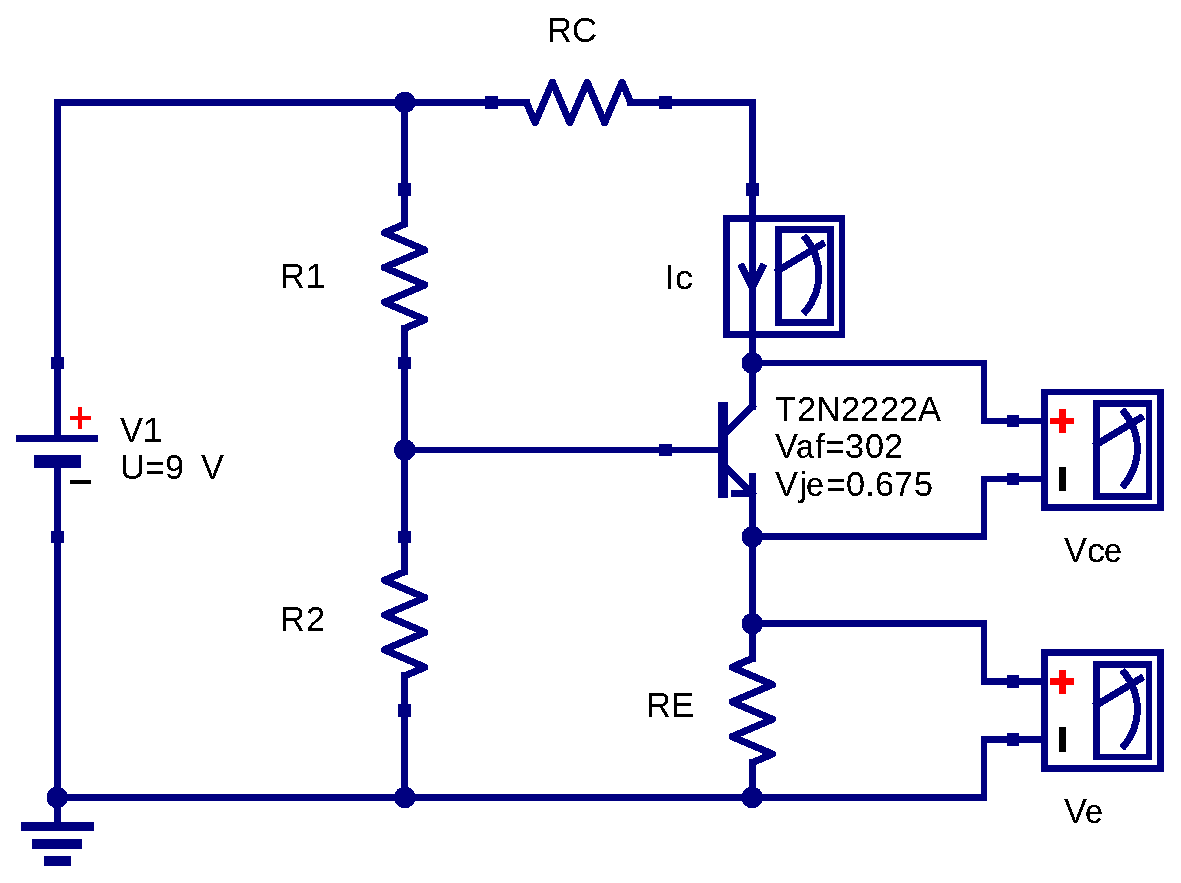
\includegraphics[scale=0.54]{diagramas/figura12.eps}
\caption{Simulación del circuito.}
\label{figura12}
\end{figure}

\begin{table}[!h]
\begin{center}
    \begin{tabular}{|c|c|c|c||c|c||c|c|}
    \hline
    $R_1[\Omega]$ & $R_2[\Omega]$ & $R_C[\Omega]$ & $R_E[\Omega]$ &
    $V_{\text{CE}}[V]$ & $V_{\text{E}}[V]$ &
    $I_{\text{C}}[\mu{A}]$ & $I_{\text{C}}[mA]$
    \tabularnewline \hline \hline
    $  1k$ & $200$ & $100$ & $22$ & $4.79$ & $0.762$ & $ 190$ & $34.5$ \tabularnewline \hline
    $4.7k$ & $ 1k$ & $200$ & $47$ & $4.71$ & $0.820$ & $93.9$ & $17.4$ \tabularnewline \hline
    \end{tabular}
\end{center}
\caption{Resultados obtenidos de la simulación.}
\label{cuadro08}
\end{table}

\subsubsection{Placa de prueba}
El circuito armado puede verse en la \textbf{figura~\ref{figura13}}, alimentado
por una fuente estable de $9[\text{V}]$.

En el circuito se fueron variando las resistencias obtenidas en el calculo
anterior, y se midieron los valores de voltaje y corriente, estos se muestran
en el \textbf{cuadro~\ref{cuadro09}}.

\begin{figure}[!h]
\centering
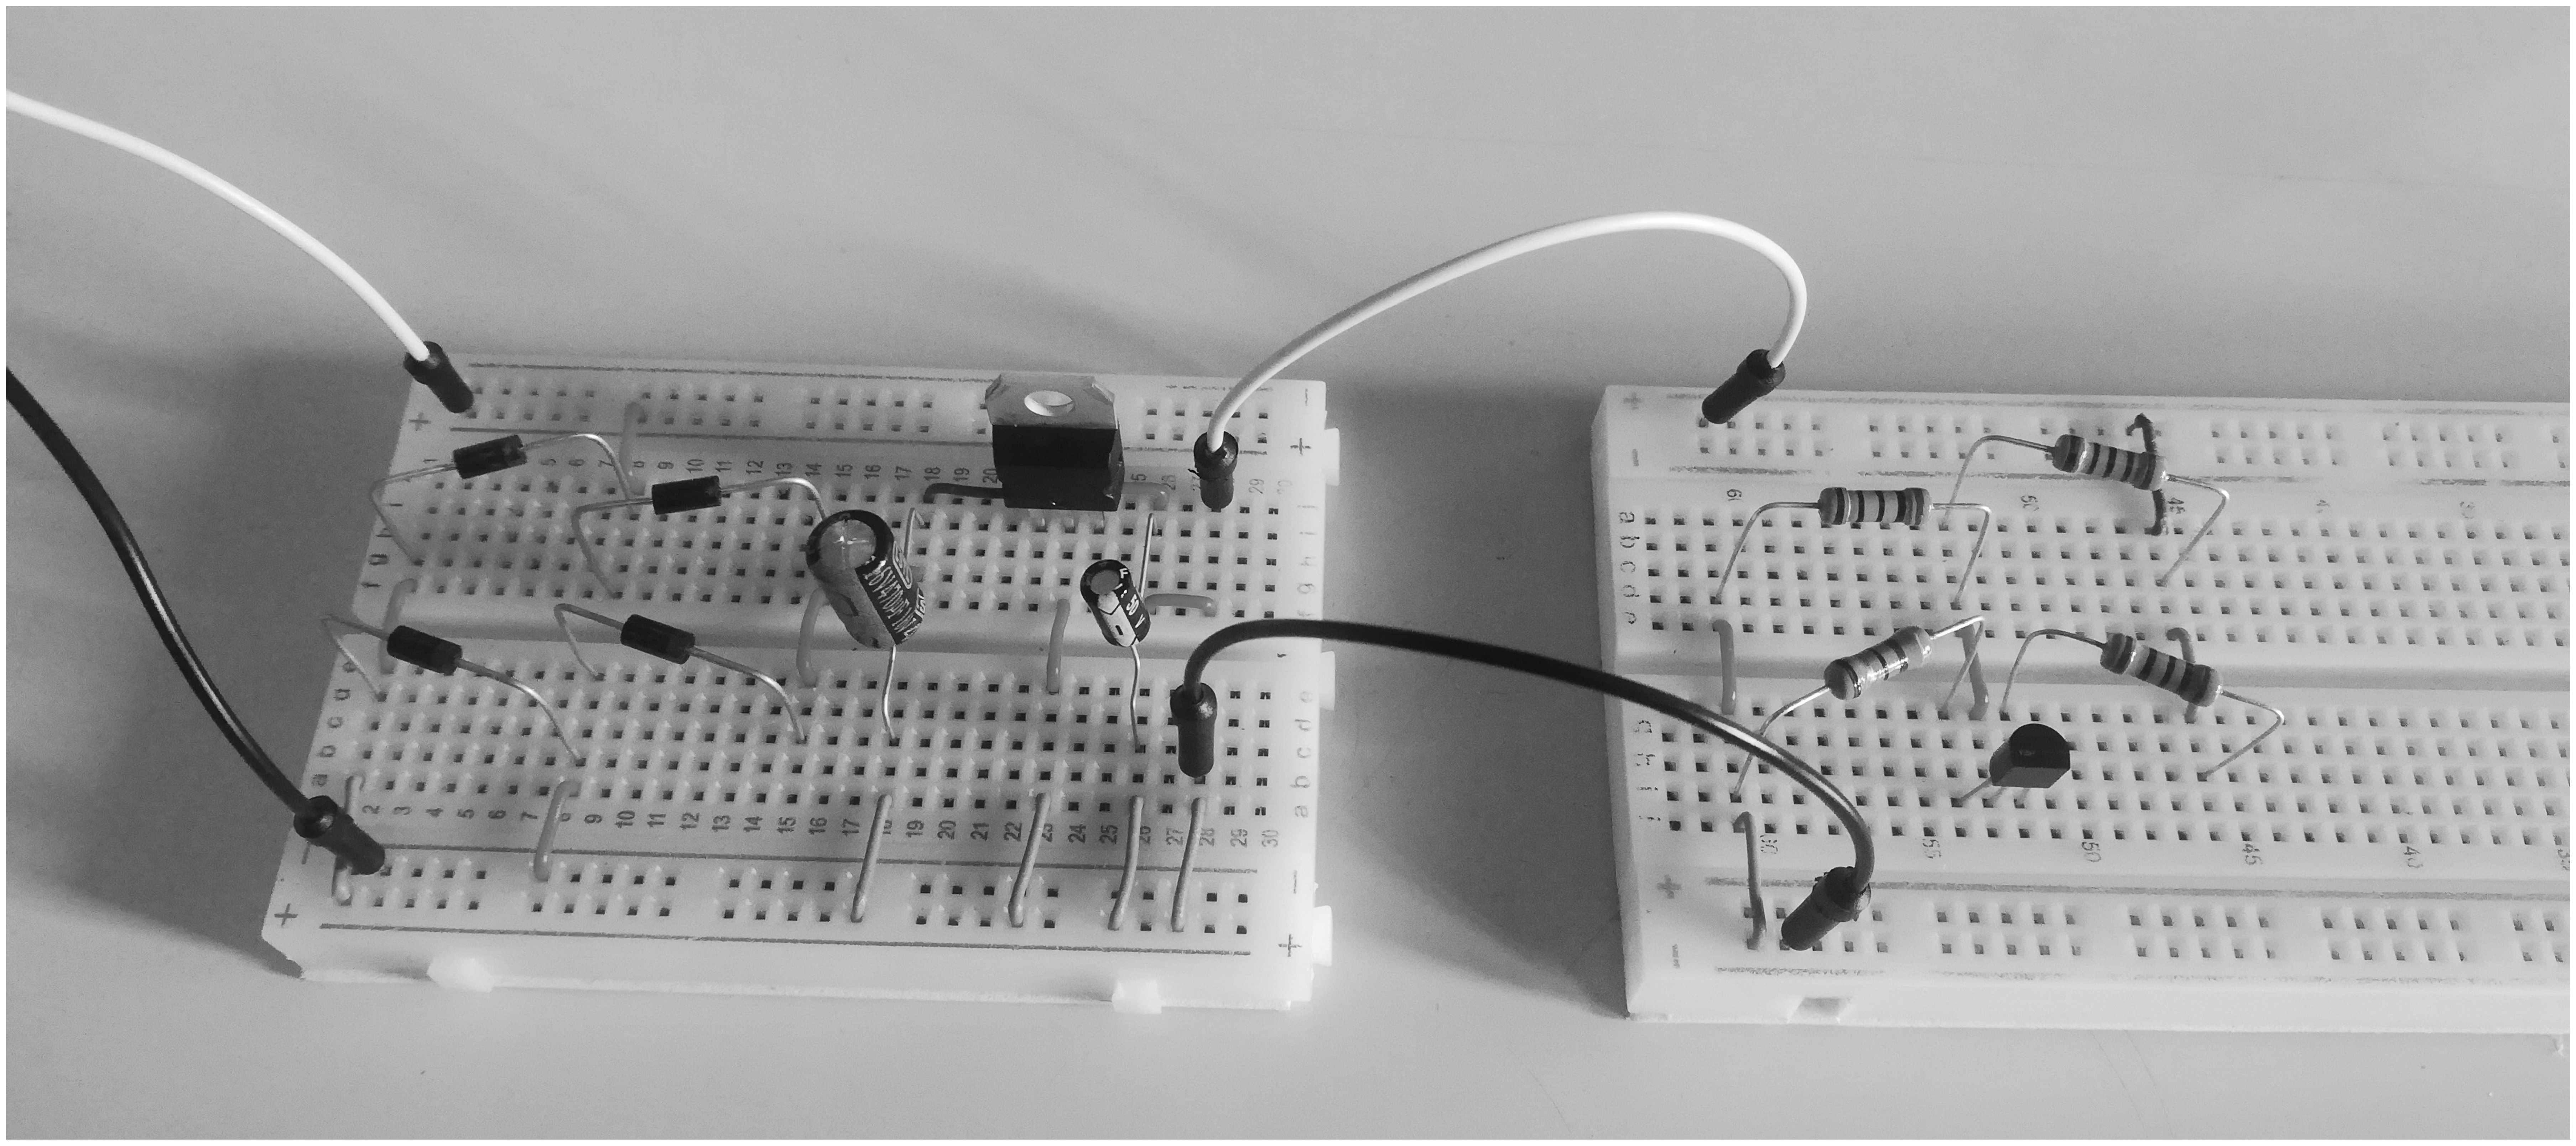
\includegraphics[scale=0.10]{diagramas/figura13.eps}
\caption{Polarización con divisor de voltaje en placa de pruebas.}
\label{figura13}
\end{figure}

\begin{table}[!h]
\begin{center}
    \begin{tabular}{|c|c|c|c||c|c||c|c|}
    \hline
    $R_1[\Omega]$ & $R_2[\Omega]$ & $R_C[\Omega]$ & $R_E[\Omega]$ &
    $V_{\text{CE}}[V]$ & $V_{\text{E}}[V]$ &
    $I_{\text{B}}[\mu{A}]$ & $I_{\text{C}}[mA]$
    \tabularnewline \hline \hline
    $ 1k$ & $ 200$ & $100$ & $22$ & $4.63$ & $0.805$ & $125.6$ & $36.6$ \tabularnewline \hline
    $10k$ & $3.3k$ & $ 47$ & $10$ & $3.01$ & $1.165$ & $ 0.03$ & $24.7$ \tabularnewline \hline
    \end{tabular}
\end{center}
\caption{Valores medidos en la placa de pruebas.}
\label{cuadro09}
\end{table}

\subsubsection{Valores de polarización}
Puede observarse que en la segunda medición los valores entre el calculo
teórico, simulación y medición real hay muchas discrepancias, por lo que se
utilizaran los valores de la primera medición. Con lo cual se halla el punto $Q$
de operación, que puede verse en la \textbf{figura~\ref{curva02}}.

\begin{figure}[!ht]
    \centering
    % GNUPLOT: LaTeX picture with Postscript
\begingroup
  \makeatletter
  \providecommand\color[2][]{%
    \GenericError{(gnuplot) \space\space\space\@spaces}{%
      Package color not loaded in conjunction with
      terminal option `colourtext'%
    }{See the gnuplot documentation for explanation.%
    }{Either use 'blacktext' in gnuplot or load the package
      color.sty in LaTeX.}%
    \renewcommand\color[2][]{}%
  }%
  \providecommand\includegraphics[2][]{%
    \GenericError{(gnuplot) \space\space\space\@spaces}{%
      Package graphicx or graphics not loaded%
    }{See the gnuplot documentation for explanation.%
    }{The gnuplot epslatex terminal needs graphicx.sty or graphics.sty.}%
    \renewcommand\includegraphics[2][]{}%
  }%
  \providecommand\rotatebox[2]{#2}%
  \@ifundefined{ifGPcolor}{%
    \newif\ifGPcolor
    \GPcolorfalse
  }{}%
  \@ifundefined{ifGPblacktext}{%
    \newif\ifGPblacktext
    \GPblacktexttrue
  }{}%
  % define a \g@addto@macro without @ in the name:
  \let\gplgaddtomacro\g@addto@macro
  % define empty templates for all commands taking text:
  \gdef\gplbacktext{}%
  \gdef\gplfronttext{}%
  \makeatother
  \ifGPblacktext
    % no textcolor at all
    \def\colorrgb#1{}%
    \def\colorgray#1{}%
  \else
    % gray or color?
    \ifGPcolor
      \def\colorrgb#1{\color[rgb]{#1}}%
      \def\colorgray#1{\color[gray]{#1}}%
      \expandafter\def\csname LTw\endcsname{\color{white}}%
      \expandafter\def\csname LTb\endcsname{\color{black}}%
      \expandafter\def\csname LTa\endcsname{\color{black}}%
      \expandafter\def\csname LT0\endcsname{\color[rgb]{1,0,0}}%
      \expandafter\def\csname LT1\endcsname{\color[rgb]{0,1,0}}%
      \expandafter\def\csname LT2\endcsname{\color[rgb]{0,0,1}}%
      \expandafter\def\csname LT3\endcsname{\color[rgb]{1,0,1}}%
      \expandafter\def\csname LT4\endcsname{\color[rgb]{0,1,1}}%
      \expandafter\def\csname LT5\endcsname{\color[rgb]{1,1,0}}%
      \expandafter\def\csname LT6\endcsname{\color[rgb]{0,0,0}}%
      \expandafter\def\csname LT7\endcsname{\color[rgb]{1,0.3,0}}%
      \expandafter\def\csname LT8\endcsname{\color[rgb]{0.5,0.5,0.5}}%
    \else
      % gray
      \def\colorrgb#1{\color{black}}%
      \def\colorgray#1{\color[gray]{#1}}%
      \expandafter\def\csname LTw\endcsname{\color{white}}%
      \expandafter\def\csname LTb\endcsname{\color{black}}%
      \expandafter\def\csname LTa\endcsname{\color{black}}%
      \expandafter\def\csname LT0\endcsname{\color{black}}%
      \expandafter\def\csname LT1\endcsname{\color{black}}%
      \expandafter\def\csname LT2\endcsname{\color{black}}%
      \expandafter\def\csname LT3\endcsname{\color{black}}%
      \expandafter\def\csname LT4\endcsname{\color{black}}%
      \expandafter\def\csname LT5\endcsname{\color{black}}%
      \expandafter\def\csname LT6\endcsname{\color{black}}%
      \expandafter\def\csname LT7\endcsname{\color{black}}%
      \expandafter\def\csname LT8\endcsname{\color{black}}%
    \fi
  \fi
    \setlength{\unitlength}{0.0500bp}%
    \ifx\gptboxheight\undefined%
      \newlength{\gptboxheight}%
      \newlength{\gptboxwidth}%
      \newsavebox{\gptboxtext}%
    \fi%
    \setlength{\fboxrule}{0.5pt}%
    \setlength{\fboxsep}{1pt}%
    \definecolor{tbcol}{rgb}{1,1,1}%
\begin{picture}(5760.00,3600.00)%
    \gplgaddtomacro\gplbacktext{%
      \csname LTb\endcsname%%
      \put(380,440){\makebox(0,0)[r]{\strut{}}}%
      \put(380,736){\makebox(0,0)[r]{\strut{}}}%
      \put(380,1032){\makebox(0,0)[r]{\strut{}}}%
      \put(380,1328){\makebox(0,0)[r]{\strut{}}}%
      \put(380,1624){\makebox(0,0)[r]{\strut{}}}%
      \put(380,1920){\makebox(0,0)[r]{\strut{}}}%
      \put(380,2215){\makebox(0,0)[r]{\strut{}}}%
      \put(380,2511){\makebox(0,0)[r]{\strut{}}}%
      \put(380,2807){\makebox(0,0)[r]{\strut{}}}%
      \put(380,3103){\makebox(0,0)[r]{\strut{}}}%
      \put(380,3399){\makebox(0,0)[r]{\strut{}}}%
      \put(500,240){\makebox(0,0){\strut{}}}%
      \put(1044,240){\makebox(0,0){\strut{}}}%
      \put(1589,240){\makebox(0,0){\strut{}}}%
      \put(2133,240){\makebox(0,0){\strut{}}}%
      \put(2677,240){\makebox(0,0){\strut{}}}%
      \put(3222,240){\makebox(0,0){\strut{}}}%
      \put(3766,240){\makebox(0,0){\strut{}}}%
      \put(4310,240){\makebox(0,0){\strut{}}}%
      \put(4855,240){\makebox(0,0){\strut{}}}%
      \put(5399,240){\makebox(0,0){\strut{}}}%
      \csname LTb\endcsname%%
      \put(5508,1523){\makebox(0,0)[l]{\strut{}$I_{\text{B}} = 125.6[\mu{A}]$}}%
      \put(5508,2623){\makebox(0,0)[l]{\strut{}$I_{\text{B}} = 244.2[\mu{A}]$}}%
      \put(935,3251){\makebox(0,0)[l]{\strut{}$0.675[V]$}}%
      \put(3113,3251){\makebox(0,0)[l]{\strut{}$4.63[V]$}}%
      \put(5508,3251){\makebox(0,0)[l]{\strut{}$9[V]$}}%
    }%
    \gplgaddtomacro\gplfronttext{%
      \csname LTb\endcsname%%
      \put(190,1919){\rotatebox{-270.00}{\makebox(0,0){\strut{}$I_{\text{C}}[mA]$}}}%
      \put(2949,140){\makebox(0,0){\strut{}$V_{\text{CE}}[V]$}}%
    }%
    \gplgaddtomacro\gplbacktext{%
      \csname LTb\endcsname%%
      \put(380,440){\makebox(0,0)[r]{\strut{}}}%
      \put(380,736){\makebox(0,0)[r]{\strut{}}}%
      \put(380,1032){\makebox(0,0)[r]{\strut{}}}%
      \put(380,1328){\makebox(0,0)[r]{\strut{}}}%
      \put(380,1624){\makebox(0,0)[r]{\strut{}}}%
      \put(380,1920){\makebox(0,0)[r]{\strut{}}}%
      \put(380,2215){\makebox(0,0)[r]{\strut{}}}%
      \put(380,2511){\makebox(0,0)[r]{\strut{}}}%
      \put(380,2807){\makebox(0,0)[r]{\strut{}}}%
      \put(380,3103){\makebox(0,0)[r]{\strut{}}}%
      \put(380,3399){\makebox(0,0)[r]{\strut{}}}%
      \put(500,240){\makebox(0,0){\strut{}}}%
      \put(1044,240){\makebox(0,0){\strut{}}}%
      \put(1589,240){\makebox(0,0){\strut{}}}%
      \put(2133,240){\makebox(0,0){\strut{}}}%
      \put(2677,240){\makebox(0,0){\strut{}}}%
      \put(3222,240){\makebox(0,0){\strut{}}}%
      \put(3766,240){\makebox(0,0){\strut{}}}%
      \put(4310,240){\makebox(0,0){\strut{}}}%
      \put(4855,240){\makebox(0,0){\strut{}}}%
      \put(5399,240){\makebox(0,0){\strut{}}}%
      \csname LTb\endcsname%%
      \put(5508,1523){\makebox(0,0)[l]{\strut{}$I_{\text{B}} = 125.6[\mu{A}]$}}%
      \put(5508,2623){\makebox(0,0)[l]{\strut{}$I_{\text{B}} = 244.2[\mu{A}]$}}%
      \put(935,3251){\makebox(0,0)[l]{\strut{}$0.675[V]$}}%
      \put(3113,3251){\makebox(0,0)[l]{\strut{}$4.63[V]$}}%
      \put(5508,3251){\makebox(0,0)[l]{\strut{}$9[V]$}}%
    }%
    \gplgaddtomacro\gplfronttext{%
      \csname LTb\endcsname%%
      \put(190,1919){\rotatebox{-270.00}{\makebox(0,0){\strut{}$I_{\text{C}}[mA]$}}}%
      \put(2949,140){\makebox(0,0){\strut{}$V_{\text{CE}}[V]$}}%
    }%
    \gplbacktext
    \put(0,0){\includegraphics[width={288.00bp},height={180.00bp}]{curva2}}%
    \gplfronttext
  \end{picture}%
\endgroup

    \caption{Punto $Q$ hallado.}
    \label{curva02}
\end{figure}

Según las pruebas realizadas los valores obtenidos son:
\begin{equation*}
    \begin{split}
        R_{\text{1}} &= 1[k\Omega]\\
        R_{\text{2}} &= 200[\Omega]\\
        R_{\text{C}} &= 100[\Omega]\\
        R_{\text{E}} &= 22[\Omega]\\
\end{split}
\end{equation*}

Ecuación de la recta de carga:
\begin{equation*}
    I_{\text{C}} = \frac{9}{122} - \frac{1}{122}V_{\text{CE}}
\end{equation*}

Punto $Q$:
\begin{equation*}
    \begin{split}
        V_{\text{CE}} = 4.63\,[\text{V}]\\
        I_{\text{C}} = 36.6\,[\text{mA}]\\
    \end{split}
\end{equation*}

Rango máximo de corriente de base:
$-107.34[\mu{\text{A}}] < I_{\text{B}} < 107.34[\mu{\text{A}}]$.

